\section{Progettazione Concettuale}
\subsection{Schema scheletro}

\subsection{Raffinamenti proposti}
Min-card tra PlayersInGame e games diventerà 0-N al posto di 1-N.
\medskip

Potremmo parlare del fatto che il color è univoco tra i giocatori di una partita ma non poteva essere messo come chiavi altrimenti un giocatore poteva potenzialmente giocare alla stessa partita con colori diversi

\subsection{Schema concettuale finale}
\clearpage
\begin{figure}[ht]
    \centerline{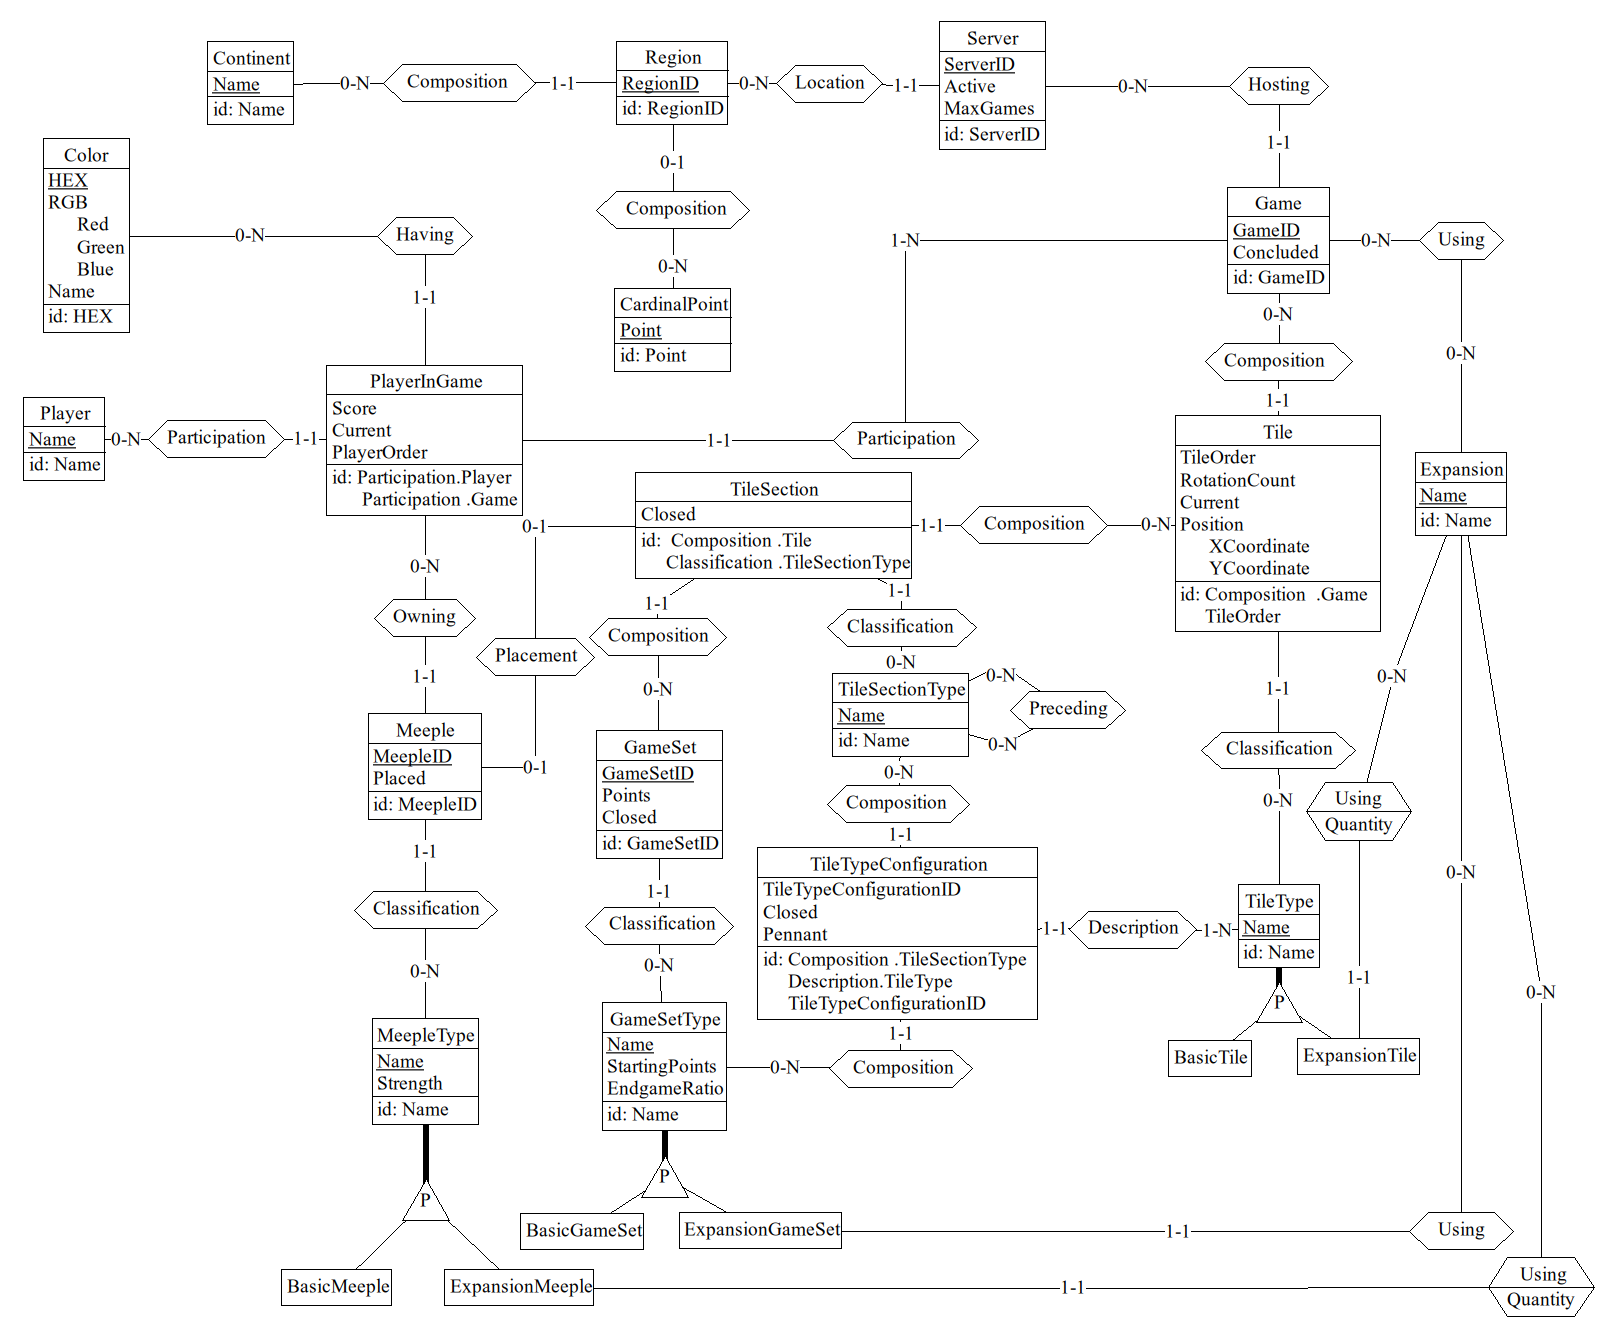
\includegraphics[scale=0.375]{images/Progettazione/Concettuale/modello.png}}
\end{figure}